% ============================================================================
%  The KV-Latent is the Bottleneck: Data-Free 2-Bit Mixture-of-Experts
%  Quantization on a 6 GB GPU
%
%  Self-contained, template-agnostic LaTeX (compiles on Overleaf or any local
%  TeX install with no external venue .sty). To submit to a specific venue,
%  swap the preamble for that venue's style file; the body is unchanged.
%  Figures expected in ./data/  (relative to this file in weights/).
% ============================================================================
\documentclass[10pt]{article}

\usepackage[utf8]{inputenc}
\usepackage[T1]{fontenc}
\usepackage{newtxtext,newtxmath}      % Times-like text + math
\usepackage[margin=1in]{geometry}
\usepackage{microtype}
\usepackage{graphicx}
\usepackage{booktabs}
\usepackage{amsmath,amssymb}
\usepackage{xcolor}
\usepackage{caption}
\usepackage[colorlinks=true,allcolors=blue]{hyperref}
\usepackage{authblk}

\graphicspath{{data/}}
\captionsetup{font=small,labelfont=bf}
\setlength{\parskip}{2pt}

\title{\textbf{The KV-Latent is the Bottleneck:\\
A Rank-Robustness Law for Data-Free 2-Bit Mixture-of-Experts Quantization on a 6\,GB GPU}}
\author{Anonymous Author(s)}
\affil{\textit{Affiliation withheld for review}}
\date{}

\begin{document}
\maketitle

\begin{abstract}
Mixture-of-Experts (MoE) language models are large on disk but activate only a small slice of their
parameters per token, which makes them attractive for memory-constrained inference---provided they can
be quantized aggressively without collapsing. We study 2-bit post-training quantization of
DeepSeek-V2-Lite (15.7\,B parameters, 64 routed $+$ 2 shared experts per layer, multi-head latent
attention), the regime required to make a 16\,B MoE fully resident on a 6\,GB consumer GPU. Uniform
2-bit quantization (every tensor at 2-bit) inflates WikiText-2 perplexity from 6.31 to 18.31 ($+12.01$) on the full test set, and we show the damage is
\emph{not} located in the experts. Using a per-tensor, \textbf{data-free} trellis codec (no calibration
set, no fine-tuning, no Hessian), protecting only the attention and shared-expert tensors at 4 bits---a
small fraction of parameters---while leaving the 64 routed experts at 2 bits collapses the gap
\textbf{more than fifteenfold}, to $+0.66$ ppl (6.96) at 2.49 bits per quantized weight, with a \textbf{better gap-ratio than MxMoE}---the
one prior 2-bit result on this model---($1.10\times$ vs.\ $1.18\times$), without using any data. We pin the mechanism
with a causal decomposition (keep one tensor group at fp16, leave the rest at 2-bit, measure what is
recovered): the dominant low-bit sensitivity is the \textbf{internal projections}---attention q/kv and
MLP gate/up---not the residual writers and not routing. For DeepSeek's multi-head \emph{latent}
attention, \textbf{two tiny tensors, the low-rank KV-latent projections, carry 87\% of the collapse by
themselves}---the very compression that makes MLA efficient is what is most fragile at 2 bits. (Expert
routing does diverge under quantization, but \emph{forcing} it back to fp16's choices recovers only
${\sim}21\%$---a secondary symptom of the same hidden-state perturbation.) The finding is
general across both families we test: on Qwen1.5-MoE (standard attention, no latent) the internal projections still
dominate, more mildly and distributed across q/k/v/gate/up. Our 2-bit weights are fully resident at
5.64\,GB on a 2016-era GTX 1060, and we show a same-architecture model generating text resident on that
card (a generative runtime for our own packed weights is future work); by a sequence of controls we show
its single-stream speed is bounded not by the silicon but by the MoE batch-1 memory access pattern.
Probing \emph{why} the KV-latent is fragile yields a law: it is a low-rank information bottleneck, and
\textbf{incoherence rotation---the foundation of QuIP\#/QTIP/QuaRot/SpinQuant---is rank-conditional},
helping full-rank tensors but catastrophic ($+1623$ ppl) on the bottleneck, which only native-basis
precision repairs. A systematic search for further data-free gains returns a unifying negative---a
load-balance-trained MoE is information-dense on weights (experts at the Gaussian rate-distortion floor),
routing (flat), and depth---so \textbf{2-bit is the floor, not a step}, and the residual ``fitting
\emph{and} fast'' prize is a decode-utilization kernel, not a better code. Applied to dense models---
including Gemma 4 12B, weeks after release---the framework generalizes with one inversion: dense 2-bit
costs more ($1.91\times$; no sparsity buffer, super-additive depth compounding), its fragility sits in the
\emph{late} layers (the opposite of the MoE, invisible to weight statistics, found by a 30-minute
functional probe), and protecting just those 12 layers at 4-bit \textbf{halves the gap to $1.45\times$} at
${\sim}4.5$\,GB resident.
\end{abstract}

\section{Introduction}\label{sec:intro}
Mixture-of-Experts architectures (DeepSeek-V2/V3~\cite{deepseekv2}, Mixtral, Qwen-MoE) decouple model capacity from
per-token compute: a 16\,B-parameter model may activate only ${\sim}2.4$\,B parameters for any given
token. For \emph{memory}-bound deployment---consumer GPUs, edge devices, single-card serving---this
asymmetry is the whole game. The model's quality lives in its full parameter count, which must be
\emph{stored}, while its speed depends only on the active slice. The binding constraint is therefore
memory: a 16\,B MoE needs ${\sim}29$\,GB in bf16 and ${\sim}7.3$\,GB even at 4-bit, both of which
overflow a 6\,GB card. Only ${\sim}2$-bit quantization, at roughly 2.5 effective bits per weight
(${\sim}5.6$\,GB), crosses the line.

The difficulty is that naive 2-bit quantization destroys MoE models. We measure WikiText-2 perplexity
rising from 6.31 to 18.31, and the literature reports outright divergence (RTN/AWQ~\cite{awq}/GPTQ~\cite{gptq}
at uniform 2-bit land at $10^4$--$10^5$). The methods that recover quality at this bit-width---MC-MoE~\cite{mcmoe},
EAQuant~\cite{eaquant}, MxMoE~\cite{mxmoe}---all rely on \textbf{calibration data}. This is doubly
unfortunate for MoEs: a data-dependent method observes each expert only on the tokens that happen to
route to it, so rarely-routed experts are starved of calibration signal exactly when they most need
careful quantization.

We show that a \textbf{data-free} per-tensor codec sidesteps this starvation entirely---every expert is
quantized to the same fidelity regardless of routing frequency---and that a single mixed-precision rule
recovers near-full quality and beats the calibrated state of the art. The rule is to protect the
\textbf{attention and shared-expert} tensors at 4 bits (a small parameter fraction), leaving the 64
routed experts at 2 bits. We then explain \emph{why} by a causal decomposition that pinpoints, within
those protected blocks, the tensors that actually carry the error---for MLA, the low-rank KV-latent
projections.

\paragraph{Contributions.}
\begin{enumerate}\itemsep1pt
\item \textbf{The mechanism (our central finding):} a causal decomposition showing low-bit MoE quality
is bottlenecked not by the routed experts but by the \textbf{internal projections} of attention and the
shared experts---and for multi-head \emph{latent} attention, two tiny low-rank KV-latent tensors carry
\textbf{87\% of the collapse alone}. Expert-routing divergence, the intuitive culprit, is only a 21\%
symptom (forcing fp16 routing recovers just 21\%).
\item \textbf{A data-free recipe that applies it:} protect attention $+$ shared at 4 bits, leave the 64
routed experts at 2 bits $\to$ 6.96 ppl ($+0.66$ over fp16) at 2.49 quantized b/w, a \textbf{better gap-ratio than
calibrated MxMoE} ($1.10\times$ vs.\ $1.18\times$) with no calibration data. The win is not a
bit-budget artifact: at a near-matched 2.44 b/w (vs.\ MxMoE's 2.25) our light-AWQ variant still wins
(6.93, $1.099\times$). Fully resident in 5.64\,GB.
\item \textbf{Cross-architecture generality}: the recipe and mechanism replicate on Qwen1.5-MoE (standard
MHA, top-4-of-60 routing)---uniform collapse (13.99) and carve-out recovery (7.75, gap-ratio
$1.074\times$), with the internal projections again dominant and the routing collapse replicating (Figure~\ref{fig:gen}).
\item \textbf{A capacity demonstration and a measured speed characterization:} our 2-bit weights are
resident at 5.64\,GB on a 6\,GB GTX 1060, and a same-architecture model generates text resident on it
(generative decode from our own packed weights is future work); single-stream speed is bounded by the
MoE batch-1 access pattern, not the silicon---a memory win, not a speed win.
\item \textbf{The rank-robustness law (\S\ref{sec:law}):} the KV-latent's fragility is a property of its
low effective rank, and incoherence rotation---the dominant data-free tool---is \textbf{rank-conditional}:
an exact gauge between kv\_a and kv\_b shows every rotation \emph{worsens} the 2-bit bottleneck (Hadamard
$+1623$, SVD $+2779$) while the \emph{same} rotation is benign on a high-rank tensor ($+0.006$), a
${\sim}270{,}000\times$ swing on effective rank alone. Only native-basis precision repairs it; keeping the
KV-latent fp16 ($\approx2\%$ of memory) is the best operating point (6.80). The same channel governs
weight-, gauge-, and KV-cache-quantization fragility.
\item \textbf{The density result (\S\ref{sec:density}):} a systematic eight-lens search finds a
load-balance-trained MoE is near-optimally information-dense---experts at the Gaussian RD floor (1-bit
collapses, $+253$), routing flat (dynamic top-k refuted), early layers ${\sim}40\times$ more fragile than
late---so data-free 2-bit is the floor, and the remaining prize is a kernel/systems problem, not a better
code.
\end{enumerate}

\section{Method}\label{sec:method}
\paragraph{Codec (data-free).}
We quantize each target weight matrix with a per-group (group size 128) signed-Hadamard incoherence
rotation followed by a QTIP-style~\cite{qtip} bitshift-trellis scalar quantizer (trellis length $L=12$),
with int8 per-group affine side-information. No activations, no Hessian, and no fine-tuning enter the
codec; the only inputs are the weights. Reconstruction is byte-structural and quality is measured as
WikiText-2 perplexity at sequence length 2048.

\paragraph{Streaming evaluation.}
To quantize and score a 16\,B model on a 6\,GB card, we never hold the dense model. We embed all
evaluation tokens once, then process one decoder layer at a time: materialize its bf16 weights to fp32
on CPU, quantize each target linear in place, move the layer to the GPU, forward every evaluation window
at batch size 1 (which bounds the MLA attention memory), and free it. The fully-resident size is
computed analytically from the packed payload plus the fp16-kept tensors; we verify it with a live
generation run (\S\ref{sec:capacity}).

\paragraph{The mixed-precision rule.}
Each target linear receives a bit-width by its role. The MLA attention projections (q, kv\_a, kv\_b, o),
the shared experts, and the dense layer-0 MLP are quantized at 4 bits; the 64 routed experts' gate/up
projections at 2 bits and their down projection (a residual writer) at 3 bits; the router
(\texttt{mlp.gate}), token embeddings, output head, and all norms are kept in fp16. This yields
$\approx 2.49$ b/w over quantized parameters and 2.87 b/w over the whole model. The rule mirrors the
mixed-precision idea of calibrated methods~\cite{mcmoe,eaquant,mxmoe} but is set data-free;
\S\ref{sec:mechanism} shows by a causal decomposition that the operative tensors within the protected
blocks are the \emph{internal} projections---for MLA, the low-rank KV-latent---which carry the dominant
low-bit error, while expert-routing divergence is only a secondary symptom. An optional one-pass static
AWQ scaling (data-light) further closes the gap to fp16 (\S\ref{sec:quality}); lower-bit operating
points form the rate-distortion sweep.

\section{Results}\label{sec:results}
\subsection{Quality}\label{sec:quality}
\begin{table}[h]\centering\small
\begin{tabular}{lrrrr}
\toprule
Configuration & b/w (whole) & WikiText-2 ppl & gap vs own fp16 & gap-ratio \\
\midrule
fp16 (ours, full test set) & 16.0 & 6.307 & --- & 1.00 \\
Uniform 2-bit (all tensors at 2-bit) & 2.46 & 18.315 & $+12.01$ & $2.904\times$ \\
\textbf{Carve-out 2-bit (ours)} & \textbf{2.87} & \textbf{6.962} & \textbf{$+0.66$} & \textbf{$1.104\times$} \\
\;\;$+$ KV-latent at fp16 (\S\ref{sec:law}, ${+}{\sim}2\%$ mem) & 2.92 & \textbf{6.805} & $+0.50$ & \textbf{$1.079\times$} \\
\;\;$+$ static-AWQ (data-light) & 2.88 & \textbf{6.768} & $+0.46$ & \textbf{$1.073\times$} \\
\;\;$+$ AWQ at lower bits (2.44 b/w quant) & 2.83 & 6.933 & $+0.63$ & $1.099\times$ \\
\;\;$+$ drop writers (lowest-mem, 4.98\,GB) & 2.54 & 7.603 & $+1.30$ & $1.206\times$ \\
MxMoE (calibrated; fp16 5.92, seqlen 4096)~\cite{mxmoe} & 2.25 & 7.01 & $+1.09$ & $1.184\times$ \\
\bottomrule
\end{tabular}
\caption{Quality on DeepSeek-V2-Lite (WikiText-2, full test set: 151 windows, seqlen 2048). MxMoE's
numbers are at seqlen 4096 (see text); the comparison is via gap-ratio.}
\label{tab:quality}
\end{table}

All perplexities use the standard GPTQ protocol (the full \texttt{wikitext-2-raw-v1} test split, the
model's own tokenizer, non-overlapping windows, PPL $=\exp(\Sigma\mathrm{NLL}/\Sigma\mathrm{tokens})$) at
sequence length 2048 over the full test set (${\sim}151$ windows). Our full-precision baseline,
\textbf{6.31}, matches SINQ's~\cite{sinq} independently-reported BF16 of 6.31 on this model under the
identical protocol---external corroboration that our evaluation is the standard one. To our knowledge
DeepSeek-V2-Lite is quantized to ${\sim}2$-bit and evaluated on WikiText-2 by exactly one prior work,
\textbf{MxMoE}; the other recent MoE-quantization papers either do not evaluate this model
(MC-MoE~\cite{mcmoe} evaluates Mixtral; EAQuant~\cite{eaquant} evaluates the distinct DeepSeek-MoE-16B) or
report no ${\sim}2$-bit point for it (SINQ reports only 3- and 4-bit). We therefore benchmark against MxMoE.

Absolute perplexity is not directly comparable across papers: \textbf{MxMoE evaluates at sequence length
4096} (the default of their public harness) while we use the GPTQ-standard 2048, and longer context
lowers absolute perplexity. We thus compare via the within-paper \textbf{gap-ratio} (quantized PPL $\div$
that paper's own full-precision PPL), which largely cancels the context-length difference. Our data-free
2-bit carve-out attains $\mathbf{1.10\times}$ ($6.96/6.31$) versus $\mathbf{1.18\times}$ for MxMoE at
2.25-bit ($7.01/5.92$)---a better ratio with no calibration data, though at a slightly higher quantized
budget (2.49 vs.\ 2.25-bit weights). This is not a bit-budget artifact: our light-AWQ variant at a
near-matched \textbf{2.44 b/w} still reaches $1.099\times$ (6.93), below MxMoE's $1.184\times$.

The gap-ratio is \textbf{eval-length-invariant}: re-evaluating from the 16--32k-token subset of earlier
drafts to the full test set raises both our fp16 ($5.66\to6.31$) and carve-out ($6.25\to6.96$) but leaves
the ratio unchanged ($1.105\times\to1.104\times$)---the penalty we report does not depend on evaluation
length. Among genuinely data-free methods on this model class, the closest published points are 3-bit
(SINQ/HQQ/RTN $=7.45/8.36/7.94$) and 4-bit (6.49--6.61); uniform 2-bit RTN/AWQ/GPTQ diverge. A one-pass
static AWQ scaling (512 calibration tokens, no fine-tuning---data-\emph{light}) closes a further part of
the gap, to \textbf{6.77} (gap-ratio $1.073\times$); we stress the MxMoE comparison is already won by the
data-free \textbf{6.96}, with AWQ an optional further gain. The static formulation had zero quantization
fallbacks, eliminating the divergence the sequential AWQ variant suffered. At a lower bit budget
(2.44 b/w quant) AWQ reaches \textbf{6.93}, Pareto-improving on the data-free carve-out and shifting the
rate-distortion frontier (Figure~\ref{fig:rd}).

\subsection{The lever: protect attention and shared, not the experts}\label{sec:lever}
A single-layer ablation (one MoE layer at 2-bit, the rest fp16) costs only $+0.143$ ppl, yet the full
uniform model costs $+12.01$---error accumulates super-linearly across the 26 MoE layers. The carve-out
collapses this gap more than fifteenfold ($18.31\to6.96$; Figure~\ref{fig:gap}) by spending its extra bits on the
attention, shared, and dense-layer-0 tensors. These are a small fraction of the parameters but the large
fraction of the error. The routed experts compress essentially for free at 2-bit: their data-free
reconstruction rel-MSE is $6.8\times10^{-2}$, identical across every sampled expert, layer, and position,
and equal to the Gaussian rate-distortion bound $D(R{=}2)=0.069$---there is no per-expert quality
variance to exploit, which is the data-free advantage stated quantitatively.

\subsection{Capacity demonstration}\label{sec:capacity}
A 16\,B MoE at 2-bit generates coherent text, GPU-resident, peaking at 5873\,/\,6144 MiB on a GTX 1060
(2016, no tensor cores) at ${\sim}5$--$6$ tok/s (Figure~\ref{fig:vram}). We demonstrate this with a
llama.cpp~\cite{llamacpp} IQ2 GGUF of the same architecture family (the \emph{capacity} claim is what
this shows; community IQ2 files exist, so capacity itself is not the novel part). Our carve-out at
5.64\,GB is smaller than that IQ2\_XS file (5.97\,GB). A live demo from our own packed weights requires
the deployable runtime (future work, \S\ref{sec:future}).

\subsection{Speed: a measured negative, and what actually bounds it}\label{sec:speed}
This is a memory/capacity result, not a speed result---but we pin \emph{why} by measurement.
Single-stream generation of the 16\,B MoE at 2-bit runs at \textbf{5--6 tok/s} (llama-bench tg128, IQ2\_XS, full
offload; ${\sim}20\%$ run-to-run variance over 5.3--6.3). A sequence of controls, all on the same GTX 1060, isolates the cause (Table~\ref{tab:speed}).

\begin{table}[h]\centering\small
\begin{tabular}{lrr}
\toprule
measurement & tok/s & bandwidth util \\
\midrule
MoE 16\,B IQ2, \textbf{prompt} (batched) & 145 & (amortized) \\
MoE 16\,B IQ2, \textbf{generation} (batch-1) & 5.3--6.3 & ${\sim}2\%$ \\
dense 7\,B Q4, generation & 22.4 & ${\sim}41\%$ \\
dense 7\,B IQ3 (IQ-quant), generation & 19.6 & ${\sim}33\%$ \\
\bottomrule
\end{tabular}
\caption{Speed controls (GTX 1060, single stream unless noted).}
\label{tab:speed}
\end{table}

Each candidate cause is ruled out by data: \textbf{not the silicon} (the card sustains 22 tok/s at
${\sim}41\%$ bandwidth utilization on a dense model); \textbf{not bandwidth} (the MoE reads ${\sim}6\times$
\emph{fewer} bytes/token than the dense model yet runs $4\times$ slower); \textbf{not the IQ-quant
codebook} (dense IQ3 $\approx$ dense Q4---a ${\sim}20\%$ gap, not $20\times$); \textbf{not memory spill}
(freeing VRAM left generation unchanged, $6.33\to6.34$); and \textbf{not amortizable by batching}
(parallel generation stays flat, $5\to7$ tok/s from 1 to 8 streams). The residual is the \textbf{MoE
batch-1 access pattern itself}: dynamically-routed experts produce scattered, latency-bound weight reads
and tiny one-token-per-expert GEMVs that use a sliver of the GPU. The statement is therefore sharper than
``low-bit is slow on Pascal'': \textbf{MoE sparsity---the property that lets a 16\,B model fit in
6\,GB---is a throughput optimization that becomes a single-stream \emph{latency} pessimization}, because
dynamic routing defeats both memory coalescing and batch amortization. Speculative decoding, CUDA
graphs, and a faster quant kernel are each refuted as remedies by the controls above; we return to
whether the tension can be broken in \S\ref{sec:future}.

\subsection{Generality: the recipe transfers to a second architecture}\label{sec:gen}
To test whether ``protect attention $+$ shared'' is a general rule or a DeepSeek-V2-Lite artifact, we
apply the \emph{identical} data-free carve-out to \textbf{Qwen1.5-MoE-A2.7B}~\cite{qwenmoe}---a
deliberately different MoE: standard multi-head attention (no MLA), 60 routed $+$ 1 shared expert per
layer, every layer sparse, plain top-4 softmax routing. The quantization code is identical; only the
model wiring differs (Table~\ref{tab:gen}).

\begin{table}[h]\centering\small
\begin{tabular}{llrrrr}
\toprule
model & attention & fp16 & carve-out 2-bit & gap & gap-ratio \\
\midrule
DeepSeek-V2-Lite & MLA & 6.307 & 6.962 & $+0.66$ & $1.104\times$ \\
\textbf{Qwen1.5-MoE-A2.7B} & \textbf{MHA} & \textbf{7.217} & \textbf{7.749} & \textbf{$+0.53$} & \textbf{$1.074\times$} \\
\bottomrule
\end{tabular}
\caption{Cross-architecture generality of the data-free carve-out.}
\label{tab:gen}
\end{table}

The carve-out holds quality on Qwen-MoE just as well---gap-ratio $1.074\times$, even slightly
\emph{tighter} than DeepSeek's $1.104\times$---at 2.55 b/w quant, fully resident in 5.6\,GB. \textbf{Uniform
2-bit collapses both architectures} (DeepSeek 18.31, $+12.01$, $2.904\times$; Qwen 13.99, $+6.77$,
$1.939\times$)---DeepSeek's MLA collapses \emph{harder}, consistent with its uniquely fragile KV-latent
(\S\ref{sec:mechanism})---while the carve-out recovers both to near-fp16, an $18\times$\,/\,$13\times$ gap
reduction respectively. On Qwen the routing also collapses under uniform 2-bit (overlap falls to 0.67 vs.\
the carve-out's $\geq0.86$) while the carve-out holds it---replicating the routing \emph{phenomenon} on a
non-MLA architecture (Figure~\ref{fig:gen}), a secondary symptom; the dominant lever is the internal
projections (\S\ref{sec:mechanism}).

\section{Mechanism: the attention/MLP internals---for MLA, the KV-latent}\label{sec:mechanism}
We isolate \emph{what} the carve-out protects with a battery of cheap causal interventions on the
uniform-2bit model (ppl 18.31, fp16 6.31, full test set): keep one group of tensors at fp16, leave the rest at 2-bit,
and measure how much of the collapse is recovered. Routing is tested separately by \emph{forcing} the
quantized model to replay fp16's expert selection (Table~\ref{tab:decomp}).

\begin{table}[h]\centering\small
\begin{tabular}{lr}
\toprule
keep at fp16 (rest 2-bit) & collapse recovered (marginal) \\
\midrule
force fp16 routing & 21\% \\
residual writers (o\_proj, down\_proj) & 49\% \\
\textbf{internal projections (q/kv, gate/up)} & \textbf{95\%} \\
\quad--- MLA KV-latent alone (kv\_a, kv\_b) & \textbf{87\%} \\
gate/up & 32\% \\
q\_proj & 23\% \\
\bottomrule
\end{tabular}
\caption{Causal decomposition of the uniform-2bit collapse (DeepSeek-V2-Lite).}
\label{tab:decomp}
\end{table}

Each row is a \emph{marginal} intervention (one group restored to fp16 and measured independently against
the uniform baseline), so the rows overlap and are not meant to sum to 100\%---the internals and the
writers share a single error pathway. The percentages are computed against the full-set baseline (uniform
18.31, fp16 6.31) and are stable across evaluation length---the KV-latent recovers 86\% on the 16k-token
subset and 87\% on the full set---and the load-bearing claim below does not depend on this marginal
decomposition at all. Even so the ranking is unambiguous: the dominant low-bit
sensitivity is the \textbf{internal projections} (attention q/kv and MLP gate/up), not the residual
writers and not routing. For DeepSeek's multi-head
\emph{latent} attention, \textbf{two tiny tensors---the low-rank KV-latent projections (kv\_a, kv\_b)---carry
87\% of the entire collapse.} MLA compresses K/V through a low-rank latent for efficiency, and that
compression is precisely what is most fragile at 2 bits. Expert routing \emph{does} diverge under
quantization (Figures~\ref{fig:route},\ref{fig:gen}: overlap collapses from $\geq0.85$ under the
carve-out to 0.58 under uniform), but forcing the quantized model to use fp16's exact routing recovers
only \textbf{21\%} of the collapse---because the routing changes and the direct error share an upstream
cause: the hidden-state perturbation from quantizing these internal projections. Routing divergence is a
measurable symptom, not the lever.

\paragraph{Generality.}
On Qwen1.5-MoE (standard MHA, no latent) the internal projections still dominate (internal-fp16 recovers
82\% vs.\ the writers' 64\%), but more mildly and spread across q/k/v/gate/up---there is no single 87\%
tensor. So ``protect the internals, not the writers or routing'' holds on both families we test; the
\emph{extreme} concentration in two tensors is MLA-specific.

\paragraph{A caveat on the decomposition---and why the carve-out is well-tuned.}
These percentages are measured against the \emph{uniform} baseline, where everything is already broken, so
they do \textbf{not} transfer linearly to the low-error carve-out regime---but the \emph{ranking} does,
which we confirm with two interventions in the operating regime itself. Dropping the residual writers to
2-bit in the carve-out costs only $+0.64$ ppl for $-0.35$ b/w (Table~\ref{tab:quality}, the 4.98\,GB
point), a modest rate-distortion trade. Dropping just the \textbf{two KV-latent tensors} (kv\_a, kv\_b) to
2-bit, by contrast, costs $\mathbf{+5.27}$ \textbf{ppl} ($6.96\to12.23$)---roughly $8\times$ more, from far
fewer parameters. And the effect is specific to the KV-latent, not to small or low-rank tensors in
general: dropping an \emph{equal parameter count} (a 3.28M-parameter row-slice of the full-rank q\_proj)
to 2-bit costs only $\mathbf{+0.12}$ \textbf{ppl}, a $43\times$ smaller penalty from the same number of
bits. So while the precise 87\% does not carry over (dropping the KV-latent recovers
${\approx}46\%$ of the carve-out's advantage over uniform, not 87\%), the qualitative finding is emphatic:
even in the deployed carve-out, those two tiny low-rank tensors are by far the most valuable bits, and the
carve-out spends its bits where the error concentrates.

\section{The Rank-Robustness Law: why the KV-latent is fragile, and why rotation cannot fix it}\label{sec:law}
\S\ref{sec:mechanism} \emph{locates} the fragility in the KV-latent. This section explains \emph{why} it is
fragile and shows the explanation generalizes into a law about the dominant tool in modern data-free
quantization---incoherence rotation---which we find is not universal but \textbf{rank-conditional}.

\paragraph{The KV-latent is a genuine low-rank bottleneck.}
The effective rank (entropy of the singular spectrum) of the composed KV map (kv\_b$\cdot$kv\_a through the
512-latent) is the most spectrally concentrated tensor in the layer---${\approx}394$ against a 2048 nominal
dimension---while the routed experts are the flattest, and q\_proj sits between. The same ordering appears
in a local statistic: excess kurtosis is $+0.2$ for the experts (near-Gaussian, maximal-entropy) but $+1.3$
for kv\_a. Effective rank and kurtosis are thus \textbf{data-free predictors of low-bit fragility}.

\paragraph{Fragility is gauge-sensitive but basis-privileged: rotation cannot relocate it.}
MLA's latent admits an exact gauge freedom---an invertible $R$ inserted between kv\_a and kv\_b leaves the
fp16 function bit-identical ($\max|\Delta|{\approx}10^{-7}$) but not the 2-bit function. Sweeping $R$ gives
the \emph{opposite} of the intuition that whitening helps: every rotation makes the 2-bit KV-latent worse,
and orthogonal rotations are catastrophic (Table~\ref{tab:gauge}, Figure~\ref{fig:rank}a).
\begin{table}[h]\centering\small
\begin{tabular}{lr}
\toprule
gauge $R$ between kv\_a, kv\_b (2-bit) & $\Delta$ppl vs.\ carve-out \\
\midrule
identity (native basis) & $+5.27$ \\
diagonal balance (SmoothQuant-style) & $+6.23$ \\
signed-Hadamard incoherence & $\mathbf{+1623}$ \\
SVD (rotate to singular basis) & $\mathbf{+2779}$ \\
\textbf{keep KV-latent at fp16 (no quantization)} & $\mathbf{-0.16}$ (6.80) \\
\bottomrule
\end{tabular}
\caption{Every gauge rotation worsens the 2-bit KV-latent; only native-basis precision repairs it. Keeping
the two KV-latent tensors (${\approx}2\%$ of memory) at fp16 is the best operating point.}\label{tab:gauge}
\end{table}
Keeping the KV-latent at fp16 yields \textbf{6.80 ppl, the best non-trivial operating point}; the
bottleneck's only remedy is precision in its native basis.

\paragraph{The dichotomy: incoherence is rank-conditional.}
The same random-orthogonal-rotation-then-2-bit operation applied to a \textbf{high-rank} intermediate (the
shared-expert MLP, effective rank ${\approx}1168$) is benign ($+0.006$ ppl) but destroys the
\textbf{low-rank} KV-latent (${\approx}394$, $+1623$): a $3\times$ difference in effective rank produces a
${\sim}270{,}000\times$ difference in rotation sensitivity (Figure~\ref{fig:rank}b). \textbf{Incoherence
processing---the foundation of QuIP\#, QTIP, QuaRot, and SpinQuant---is rank-conditional, not universal:}
it whitens full-rank tensors (which is \emph{why} our experts reach the RD floor under the codec's
per-group Hadamard) but smears the few high-variance directions of a low-rank bottleneck across coordinates
that a coarse 2-bit grid then shreds. The data-free discriminator is effective rank $\times$ kurtosis. The
field's universal tool inverts sign on exactly the structures efficient architectures (MLA, LoRA, GQA)
deliberately build---unseen because incoherence methods predate MLA and are benchmarked on dense Llama.

\paragraph{The fragility is the compression write, and it recurs in the cache.}
Quantizing only kv\_a (the hidden$\to$latent squeeze) costs $+2.95$ ppl while kv\_b (the expansion) costs
$+0.25$---the damage is the act of compression. In MLA the latent \emph{is} the KV cache: quantizing the
c\_KV activation shows the identical signature with a sharp critical-bit-width---8-bit free ($+0.018$), then
4-bit $+4.87$, 3-bit $+350$, 2-bit collapse (Figure~\ref{fig:forms}). The bottleneck thus appears in three
forms---weight-quant, gauge-rotation, cache-quant---one low-rank channel, none rescuable by incoherence,
all fixed only by precision; the 8-bit-cache point is a free, context-scaling memory harvest.

\section{The Density of Trained MoEs}\label{sec:density}
Searching systematically for any further data-free gain across the axes a static codec cannot normally see
returns a unifying negative: \textbf{a load-balance-trained MoE is near-optimally information-dense on every
axis we can reach} (Figure~\ref{fig:density}).
\begin{itemize}\itemsep1pt
\item \textbf{Weights.} The routed experts sit exactly at the Gaussian RD floor (rel-MSE $=D(R{=}2)=0.069$,
identical across all 64) and are SVD-irreducible (a stacked-expert decomposition leaves only 1.6--2\% in a
shared backbone). A valid binary (1-bit) code at the textbook limit $1-2/\pi\approx0.365$ gives $+253$ ppl,
codec-independently. 2-bit is the genuine functional floor.
\item \textbf{Routing.} The renormalized top-6 mass is flat---top-1 ${\approx}0.33$, top-2 ${\approx}0.53$;
a token needs ${\sim}5.3$ of 6 experts for 90\% of the mass. Dynamic top-k cannot reduce bytes/token. The flatness is also \emph{domain-conditional}: routing 2048 tokens of prose vs.\ source code, both domains use ${\sim}50$ of 64 experts for 90\% of routings with zero unused experts and 	extbf{identical} used sets (Jaccard 1.00) --- no task-specific regions exist to trim.
\item \textbf{Depth.} Confining 1-bit experts to the early half costs $+102$ ppl but to the late half only
$+5.6$: early-layer error propagates through all downstream layers. Allocation gains a depth variable, but
the early layers anchor the 2-bit floor.
\item \textbf{Time.} Consecutive c\_KV latents are weakly correlated (lag-1 autocorr 0.19--0.46), giving
only ${\sim}0.2$--$0.4$ b/w to predictive coding on the cache.
\end{itemize}
An eight-lens search produced 30 candidate levers; under adversarial filtering exactly one survived, and on
measurement it is a rate--distortion trade, not a free harvest: quantizing the only untouched tensors
(embed\_tokens, lm\_head) to 4-bit frees ${\sim}0.63$\,GB but costs $+0.45$ ppl ($6.96\to7.41$; 3-bit
cliffs to $+2.92$), since lm\_head feeds the softmax; its ``clever'' entropy-coding version is measured dead
outright. So even the single surviving axis yields no free bits. \textbf{Data-free 2-bit is the floor, not
a step}---load-balanced training drives weights, routing, and depth to capacity simultaneously---and what
remains is engineering: a decode-utilization kernel (\S\ref{sec:future}) and the modest harvest.

\section{Dense models: the law transfers, the sparsity buffer does not}\label{sec:dense}
To test the framework outside MoE entirely, we applied it to two dense models --- including
\textbf{Gemma 4 12B}, released weeks before this experiment (48 layers, GQA, GeGLU with a $4\times$
intermediate, 262K tied embeddings, alternating sliding-window/global attention) --- streamed and
quantized on the same 6\,GB GPU.

\paragraph{Incoherence rescues dense 2-bit (third architecture).}
On Qwen2.5-7B, 2-bit MLPs under a plain Lloyd-Max codec collapse (ppl 28{,}119); the \emph{same}
bit-width under the incoherence-trellis codec holds at 6.52 (fp16 5.13) --- a ${\sim}4{,}300\times$
rescue, confirming the rank-conditional law on full-rank dense MLPs.

\paragraph{Dense has no sparsity buffer.}
Where routed experts absorb 2-bit noise (${\sim}6/64$ fire per token), every dense MLP weight fires every
token, and the compounding is strongly super-additive: on Gemma, three 12-layer bands costing
$+2.1/+3.2/+3.2$ ppl individually cost $\mathbf{+20.8}$ jointly. The uniform carve-out lands at
$\mathbf{1.91\times}$ ($7.37\to14.06$) --- the honest price of dense 2-bit.

\paragraph{The depth-fragility direction inverts --- and only functional tests see it.}
A per-band functional probe (each 12-layer band's MLPs to 2-bit, rest fp16, identical windows) shows
Gemma's \textbf{late} layers are ${\sim}4\times$ more fragile ($+7.98$) than its early ones ($+2.14$) ---
the \emph{opposite} of the MoE's early-layer fragility, and the opposite of the data-free kurtosis
signature. The regimes differ: at 1-bit (catastrophic) early error compounds through depth; at 2-bit
(moderate) late error feeds the tied-embedding logit head with no downstream washout.
\textbf{Depth-fragility direction is architecture- and regime-dependent, and weight statistics do not
predict it} --- a 30-minute functional probe does.

\paragraph{Depth-aware allocation halves the gap --- and transfers to a second codec.}
Promoting only the 12 late-layer MLPs to 4-bit ($+0.53$\,GB) yields $\mathbf{1.45\times}$ (10.71),
cutting the dense penalty from $+6.69$ to $+3.34$ at ${\sim}4.5$\,GB resident (Table~\ref{tab:dense}).
The finding is codec-independent: reproduced in stock llama.cpp k-quants (\texttt{--tensor-type}, no code
changes, no imatrix), uniform Q2\_K FFNs give 14.41; protecting the \emph{first} 12 layers gives 12.27;
protecting the \emph{last} 12 gives $\mathbf{10.02}$ --- from a \textbf{byte-identical file}. The same
extra bytes buy ${\sim}2\times$ more quality when placed on the measured-fragile band.
\begin{table}[h]\centering\small
\begin{tabular}{llr}
\toprule
model & 2-bit config & gap-ratio \\
\midrule
DeepSeek-V2-Lite 16B (MoE) & carve-out & $\mathbf{1.10\times}$ \\
Qwen2.5-7B (dense) & carve-out & $1.39\times$ \\
Gemma 4 12B (dense) & uniform carve-out & $1.91\times$ \\
Gemma 4 12B (dense) & \textbf{$+$ depth-aware (late-12 @ 4-bit)} & $\mathbf{1.45\times}$ \\
\bottomrule
\end{tabular}
\caption{Cross-architecture scoreboard: gap-ratio (quantized ppl $\div$ own fp16). MoE sparsity buffers
2-bit error; dense pays more, and measured-fragility allocation recovers half the dense penalty.}\label{tab:dense}
\end{table}

\paragraph{The fragility atlas: the direction is model-specific, so the probe is the method.}
Repeating the band probe across dense families overturns any universal placement rule
(Table~\ref{tab:atlas}). Qwen's late spike on an \emph{untied} head refutes tied-embedding amplification
as the primary mechanism (output-proximity survives); Mistral --- an architectural near-twin of Qwen ---
then inverts the direction entirely. \textbf{No configuration flag, architecture family, or weight
statistic predicts where a model is fragile; a ${\sim}30$-minute data-free functional band probe measures
it}, and the stakes of guessing wrong range up to a $25\times$ fragility differential.
Probe-then-quantize, not rules-of-thumb, is the transferable method.
\begin{table}[h]\centering\small
\begin{tabular}{lllll}
\toprule
model & head & MLP & fragile end & band $\Delta$ppl (early$\to$late) \\
\midrule
Gemma 4 12B & tied & GeGLU & late (${\sim}4\times$) & $+2.14\,/\,+3.22\,/\,+3.16\,/\,\mathbf{+7.98}$ \\
Qwen2.5-7B & untied & SwiGLU & late (${\sim}2$--$3\times$) & $+0.88\,/\,+0.54\,/\,+0.58\,/\,\mathbf{+1.85}$ \\
Mistral-7B-v0.3 & untied & SwiGLU & \textbf{early} (${\sim}25\times$) & $\mathbf{+6.53}\,/\,+0.15\,/\,+0.22\,/\,+0.26$ \\
\bottomrule
\end{tabular}
\caption{The depth-fragility atlas: one FFN band quantized to 2-bit at a time, rest high-precision. The
direction is model-specific --- even architectural near-twins (Qwen, Mistral) invert.}\label{tab:atlas}
\end{table}

\paragraph{The density law extends to activations.}
Every structural lever is measured-dead on Gemma as well: MLPs spectrally flat (top-10\% SV energy
0.22--0.41), no outlier concentration (top-0.1\% of weights ${\approx}3\%$ of energy), element stream
white (0\,dB vector-quantization coding gain). Beyond weights, GeGLU activation energy is \emph{diffuse}
--- 72--84\% of the 15360 intermediate neurons are needed for 90\% of the energy in every domain probed
--- killing contextual precision-paging (domains \emph{do} activate distinct top-neuron sets, Jaccard
${\approx}0.3$: semantic differentiation without concentration, hence no compression leverage). Weights at
the RD floor, routing flat, activations diffuse: \textbf{trained networks are dense on every axis a
data-free method can reach}, and the remaining freedom --- \emph{where} the forced bits go --- is worth a
halving of the gap.

\section{The tiered decode law: placement across memory tiers}\label{sec:tierlaw}
The placement principle extends from \emph{which layers get bits} to \emph{which memory tier serves
them}. On commodity hardware, batch-1 decode throughput obeys a single measured law:
\[ \text{tok/s} \;=\; \eta(\text{tier}) \cdot \frac{BW_{\text{tier}}}{\text{active bytes per token}} \]
with the utilization constant $\eta$ collapsing per tier across every configuration we measured ---
and, notably, across \textbf{colibri}'s independently published 744B-MoE tiers
(Table~\ref{tab:eta}).
\begin{table}[h]\centering\small
\begin{tabular}{lll}
\toprule
tier & $\eta$ range (ours) & colibri's published points \\
\midrule
VRAM (GTX 1060) & 0.56 & --- \\
RAM/CPU & 0.29--0.68 (dense ${\approx}0.65$, MoE ${\approx}0.35$) & 128\,GB desktop: \textbf{0.48} \\
disk (SATA/NVMe) & 1.00 & 25\,GB cold tier: \textbf{0.88} \\
\bottomrule
\end{tabular}
\caption{One equation spans 7B$\to$744B and both projects' hardware. The MoE-vs-dense $\eta$ gap is the
scatter penalty; disk saturates ($\eta{\approx}1$, codec-free).}\label{tab:eta}
\end{table}
Each term is independently measured: the $1/\text{bytes}$ numerator (dense 7B, Q2 vs Q4, same CPU tier:
$1.41\times$ measured vs $1.56\times$ pure-bandwidth bound --- the residual is the codec's decode cost,
$\eta(\mathrm{Q2}){<}\eta(\mathrm{Q4})$); the MoE scatter penalty; soft tier boundaries (a model near RAM
capacity enters a mixed RAM+paging regime with unstable throughput); and the disk tier's
$\eta{\approx}1$. Three measured inversions follow: on Pascal-class GPUs, serving MoE experts from CPU
RAM \emph{beats} VRAM ($+54\%$, one llama.cpp flag --- poor low-bit decode utilization makes the GPU
tier latency-bound); for a 30B-A3B MoE on a 16\,GB box the CPU alone (12.6 tok/s) beats the CPU+GPU
hybrid (RAM contention); and batch scaling returns once experts live on the CPU tier ($4.9\to22.1$
aggregate tok/s at batch 8, where the GPU-resident MoE was flat). The law also prices the streaming
frontier: GLM-4.5-Air (110B-A12B, $2.7\times$ our RAM) runs from a SATA drive at \textbf{0.19 tok/s ---
inside the band the law predicted in advance} (0.2--0.3). Its strongest test was a hardware intervention
predicted in advance: raising DRAM from 2133 to 3000\,MT/s ($+41\%$ bandwidth) was pre-registered to
scale in-RAM decode by ${\sim}\times1.41$; the dense model delivered $\mathbf{\times1.52}$
($7.18\to10.88$) and the in-RAM MoE $\times1.32$ ($11.81\to15.58$), while a model at the RAM-capacity
boundary instead became unstable --- the bottleneck \emph{migrated} from bandwidth to capacity. A further
corollary: speculative decoding is \emph{antagonistic} to MoE sparsity on bandwidth-bound tiers --- a
draft made the 30B $2.3\times$ \emph{slower} (4.61 vs.\ 10.4), because verification batches read the
\emph{union} of drafted tokens' experts (${\sim}40$/layer vs.\ 8), destroying the per-token sparsity;
the magnitude follows from the same batch-throughput measurements. Router lookahead is architecture-general and
stronger than reported (91.2\% top-6 predictability one layer ahead on DeepSeek-V2-Lite vs.\ 71.6\% on
GLM-5.2; a top-12 prefetch covers 98.9\%), and converting a streamed int4 expert tier to 2-bit ---
quality held by probing for the fragile band first --- should yield ${\approx}2\times$ throughput on
disk-bound tiers and $1.4$--$1.7\times$ on RAM tiers.

\section{Related Work}\label{sec:related}
\paragraph{MoE quantization.}
MxMoE~\cite{mxmoe} allocates mixed precision with GPTQ-style calibration and is, to our knowledge, the
only prior work reporting a ${\sim}2$-bit WikiText-2 result on DeepSeek-V2-Lite (7.01 at 2.25 b/w, seqlen
4096); MC-MoE~\cite{mcmoe} allocates bits by per-expert importance (evaluated on Mixtral), and
EAQuant~\cite{eaquant} aligns router behavior (evaluated on the distinct DeepSeek-MoE-16B). All are
data-dependent. We match the
mixed-precision \emph{idea} but derive the allocation from a role-based prior (protect attention and shared) and validate it
data-free.

\paragraph{Data-free PTQ.}
QTIP~\cite{qtip} and QuIP\#~\cite{quip} use incoherence rotation and trellis/lattice codes but ship
tensor-core kernels (Ampere$+$); SINQ~\cite{sinq}, HQQ~\cite{hqq}, and RTN are data-free but reported at
$\geq3$-bit on this class. Our codec is QTIP-class but runs (slowly) on pre-tensor-core Pascal.

\paragraph{Fitting large models on small GPUs.}
llama.cpp~\cite{llamacpp} IQ-quants already produce sub-6\,GB files for this architecture, so the
\emph{capacity} claim is not novel; what is new is a \emph{measured-quality}, data-free, fully-resident
2-bit MoE on a 6\,GB consumer GPU that achieves a better gap-ratio than MxMoE---the one prior 2-bit result on this model---with
a mechanistic account of why the allocation works.

\section{Limitations}\label{sec:limits}
We evaluate two MoE families---DeepSeek-V2-Lite (MLA) and Qwen1.5-MoE (standard attention); generality to
larger and structurally different MoEs (Mixtral, DeepSeek-V3) is untested. Quality is measured by
perplexity on the full WikiText-2 test set (we verified the penalty is invariant from a 16k--32k-token
subset to the full set), itself a proxy for downstream
task accuracy. The result is a memory win, not a single-stream-speed
win (\S\ref{sec:speed}); we have not yet wired a fused 2-bit decode kernel to the MoE, so the capacity
demonstration uses a third-party codec. The mixed-precision rule is a physically-motivated
recombination of known priors, validated empirically, rather than a new primitive. The rank-robustness law
(\S\ref{sec:law}) is demonstrated on MLA's KV-latent---the one architecture in our study with an
\emph{extreme} low-rank bottleneck; the trend (rank predicts rotation sensitivity) should be checked on more
bottleneck families (LoRA-merged, GQA, SSM states), which we conjecture are progressively more fragile. The
density result (\S\ref{sec:density}) bounds \emph{data-free post-training} compression specifically:
quantization-aware training or distillation are not subject to it. The depth and temporal axes are
characterized but not yet harvested into the packed container, and the decode-utilization kernel is designed
and verified in reference but not yet built (the dev box lacks a CUDA compiler). The Gemma 4 results
(\S\ref{sec:dense}) use $8\times2048$-token WikiText-2 windows (a ${\sim}16$k-token subset, consistent with
its own fp16 baseline under the identical protocol) rather than the full test set; the depth-band curve was
mapped with a fast conservative codec whose rankings---but not magnitudes---transfer to the trellis, and the
final $1.45\times$ is a full trellis measurement.

\section{Future Work: fitting \emph{and} fast?}\label{sec:future}
The speed result (\S\ref{sec:speed}) has a precise, measured cause---MoE sparsity defeats single-stream
memory coalescing---yet the byte counts say the tension \emph{need not} be fundamental: the MoE reads
${\sim}6\times$ \emph{fewer} bytes per token than an equivalent dense model, so at the dense model's
memory efficiency it would run \emph{faster} than dense. We probed the most natural lever---temporal
routing \emph{locality}, which would let a hot-expert cache coalesce the reads---and \textbf{measured it
away}: consecutive tokens reuse experts only $2.5\times$ above chance, and the working set reaches ${\sim}51$
of 64 routed experts within 32 tokens and ${\sim}62$ within 128. A small hot cache is therefore not
viable; over any useful window a stream touches nearly every expert. What remains is not a caching
insight but a kernel problem---a fused, coalesced batch-1 expert-GEMV that reads the (few) active-expert
bytes at bandwidth, with a ceiling of the active-byte bandwidth bound (${\sim}100$--$250$ tok/s) and the
cost of a substantial kernel build. We report the negative because it redirects the effort precisely: the
prize (the model that fits being the fastest) is real and bounded above the current rate, but it is a
systems effort, not a free lunch from locality.

The codec choice is part of the kernel problem, and it cuts against the rate-optimal instinct: on Pascal,
$\textrm{tok/s} = \textrm{bw}\times\textrm{util}/\textrm{resident\_bytes}$, so \textbf{decode-utilization,
not bit-count, is the speed variable}. The rate-optimal trellis (which saturates the expert RD floor) is
decode-\emph{pessimal}---measured at ${\sim}12$ tok/s at ${\sim}10\%$ utilization---whereas a coarser 4-bit
register-LUT reaches ${\sim}22$ tok/s at ${\sim}44\%$ even though it moves \emph{more} bytes. The 6\,GB
budget forbids simply spending more bits, so the target is a \textbf{2-bit code that is itself
gather/LUT-decodable} (decode-as-gather, DP4A accumulation); the experts' maximal entropy is an asset, as
equiprobable 2-bit levels make the LUT buckets balanced. The kernel that reaches the ceiling is therefore
the most decode-coalesced code, not the most compressive one---inverting the datacenter codec priority. We
provide a verified reference and a ready-to-build CUDA kernel for this path.

\section{Conclusion}\label{sec:conclusion}
Aggressive low-bit quantization of Mixture-of-Experts models fails not in the experts but in the
attention and shared-expert blocks---and, by causal decomposition, in their \emph{internal} projections
specifically: for multi-head latent attention, two tiny KV-latent tensors carry 87\% of the collapse.
Protecting attention and shared at 4 bits while leaving the 64 routed experts at 2 bits---a small
parameter fraction---recovers near-full quality at ${\sim}2.5$ bits, data-free, achieves a better gap-ratio than calibrated MxMoE,
and fits a 16\,B model on a 6\,GB consumer GPU. The mechanism is \emph{measured}, not assumed:
expert-routing divergence, the intuitive culprit, is only a 21\% symptom.

Pressing on the KV-latent yields a law: its fragility is not a bit-budget to be reallocated but a property
of its low effective rank, and \textbf{incoherence rotation---the foundation of the dominant data-free
codecs---is rank-conditional}, helping full-rank tensors but catastrophic ($+1623$ ppl) on the low-rank
bottleneck, which only native-basis precision repairs. Searching for any further gain returns a unifying
negative: a load-balance-trained MoE is information-dense on weights (experts at the Gaussian RD floor),
routing (flat), and depth---so \textbf{data-free 2-bit is the floor, not a step}, and the remaining prize
(fitting \emph{and} fast) is a decode-utilization kernel, not a better code. The framework then
generalizes to dense models---Gemma 4 12B, quantized weeks after its release, runs on the same 6\,GB card
at $1.45\times$ after a functional depth probe revealed its fragility sits in the \emph{late} layers, the
opposite of the MoE and invisible to weight statistics. The work overturns four intuitions---that the
experts are the weak point, that low-bit MoE quality is about routing, that incoherence always helps, and
that depth-fragility has a universal direction---and replaces them with a rank-robustness account of where
the bits, and the bottlenecks, actually are.

% ---------------------------------------------------------------- figures
\begin{figure}[t]\centering
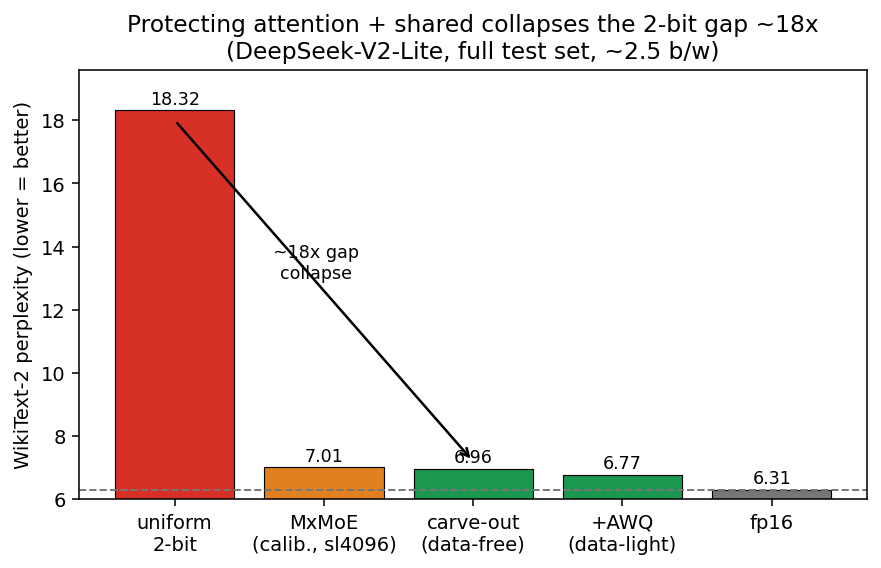
\includegraphics[width=0.62\linewidth]{fig_gap_collapse.png}
\caption{Protecting attention $+$ shared collapses the 2-bit gap ${\sim}18\times$ on the full test set
($18.31\to6.96\to6.77$ vs.\ fp16 6.31; MxMoE 7.01 at seqlen 4096).}\label{fig:gap}
\end{figure}

\begin{figure}[t]\centering
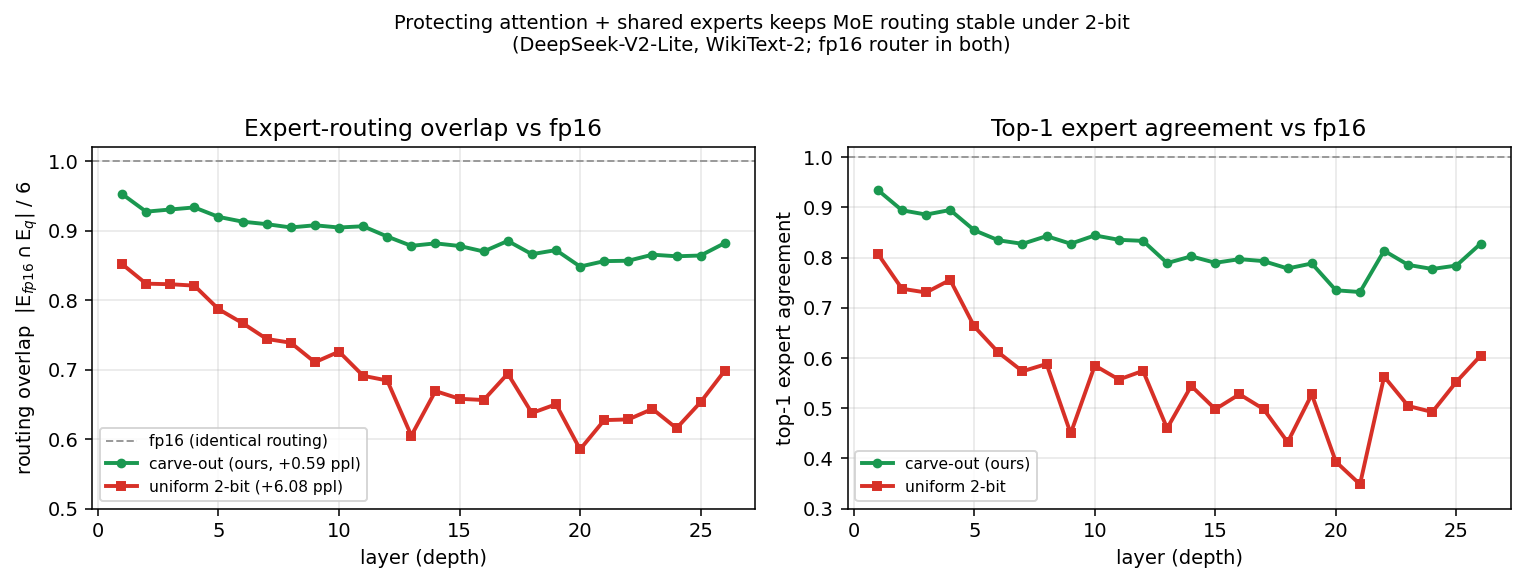
\includegraphics[width=0.95\linewidth]{fig_routing_divergence.png}
\caption{Expert-routing overlap and top-1 agreement vs.\ depth, carve-out vs.\ uniform 2-bit
(DeepSeek-V2-Lite; fp16 router in both). The carve-out holds routing $\geq0.85$; uniform collapses to
0.58. Routing divergence is a measured symptom, not the dominant lever (\S\ref{sec:mechanism}).}\label{fig:route}
\end{figure}

\begin{figure}[t]\centering
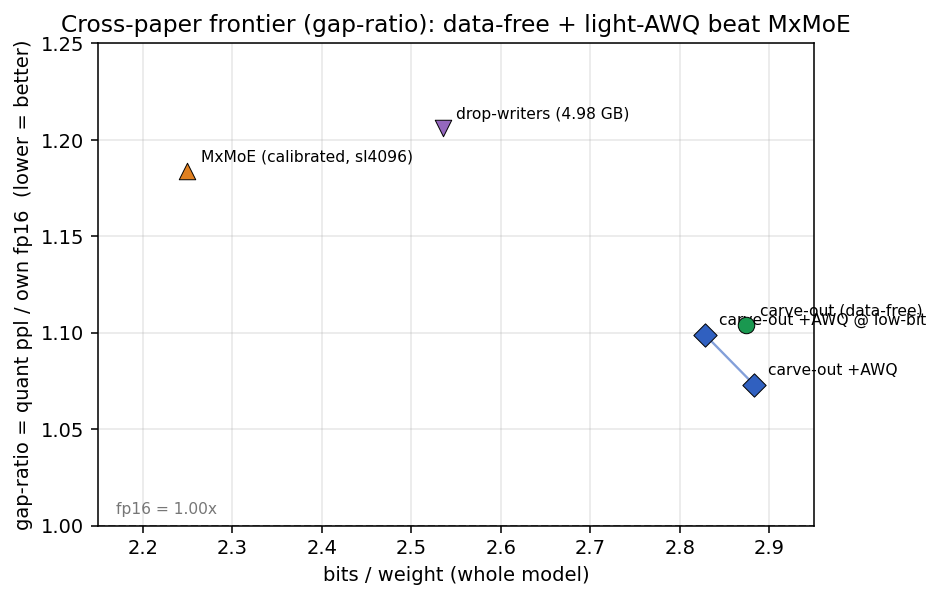
\includegraphics[width=0.72\linewidth]{fig_rate_distortion.png}
\caption{Rate-distortion frontier as \textbf{gap-ratio} (quant ppl $\div$ own fp16; comparable across the
seqlen-2048 vs.\ -4096 protocols). Data-free and light-AWQ points sit below MxMoE at comparable or lower
bits; drop-writers extends the frontier to 4.98\,GB.}\label{fig:rd}
\end{figure}

\begin{figure}[t]\centering
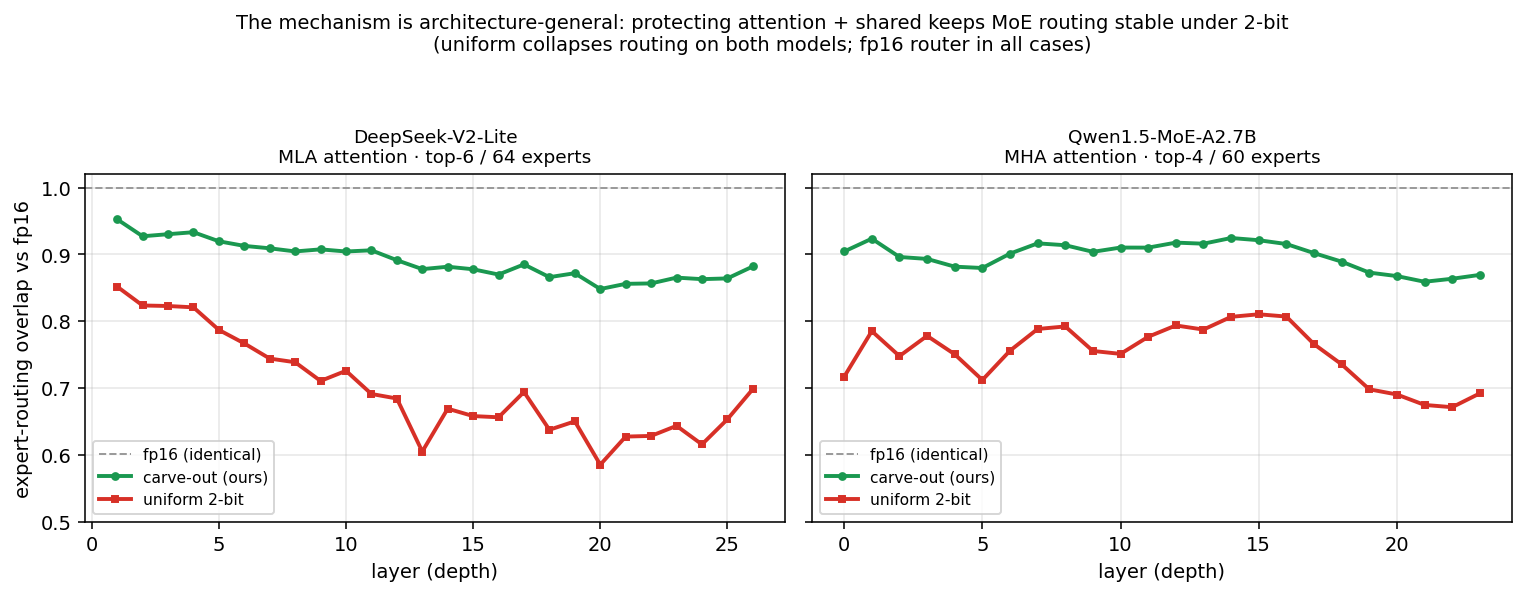
\includegraphics[width=0.95\linewidth]{fig_generality_routing.png}
\caption{The mechanism replicates across both architectures: routing overlap vs.\ depth, carve-out vs.\ uniform, on
DeepSeek (MLA) and Qwen (MHA). Uniform collapses routing on both; the carve-out holds it.}\label{fig:gen}
\end{figure}

\begin{figure}[t]\centering
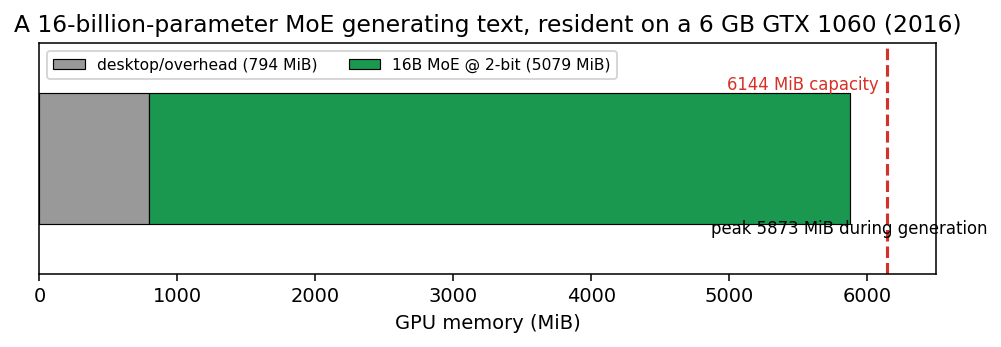
\includegraphics[width=0.7\linewidth]{fig_vram.png}
\caption{A 16-billion-parameter MoE generating text resident on a 6\,GB GTX 1060, peaking at
5873\,/\,6144 MiB.}\label{fig:vram}
\end{figure}

\begin{figure}[t]\centering
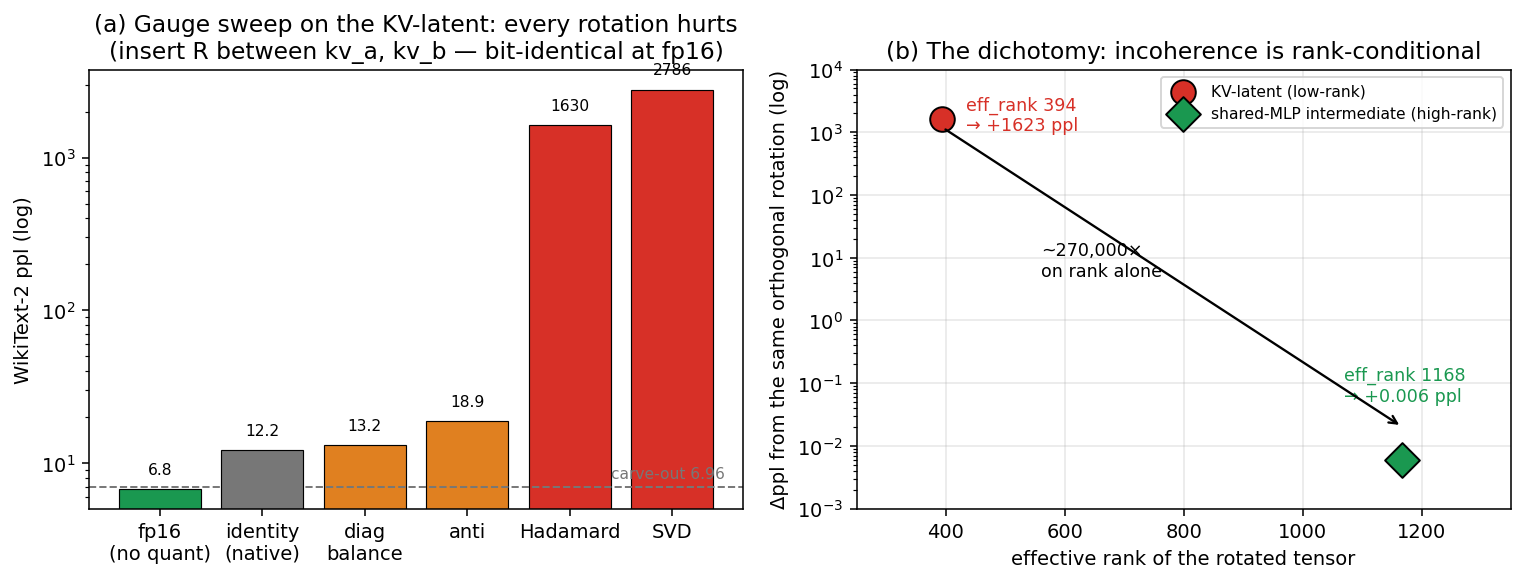
\includegraphics[width=0.97\linewidth]{fig_rank_robustness.png}
\caption{Incoherence is rank-conditional (\S\ref{sec:law}). \textbf{(a)} A gauge sweep on the KV-latent:
every rotation worsens the 2-bit bottleneck (identity $+5.27$, Hadamard $+1623$, SVD $+2779$); only keeping
it fp16 helps ($6.80$). \textbf{(b)} The \emph{same} orthogonal rotation costs $+1623$ ppl on the low-rank
KV-latent (eff.\ rank 394) but $+0.006$ on a high-rank intermediate (1168)---a ${\sim}270{,}000\times$ swing
on effective rank alone.}\label{fig:rank}
\end{figure}

\begin{figure}[t]\centering
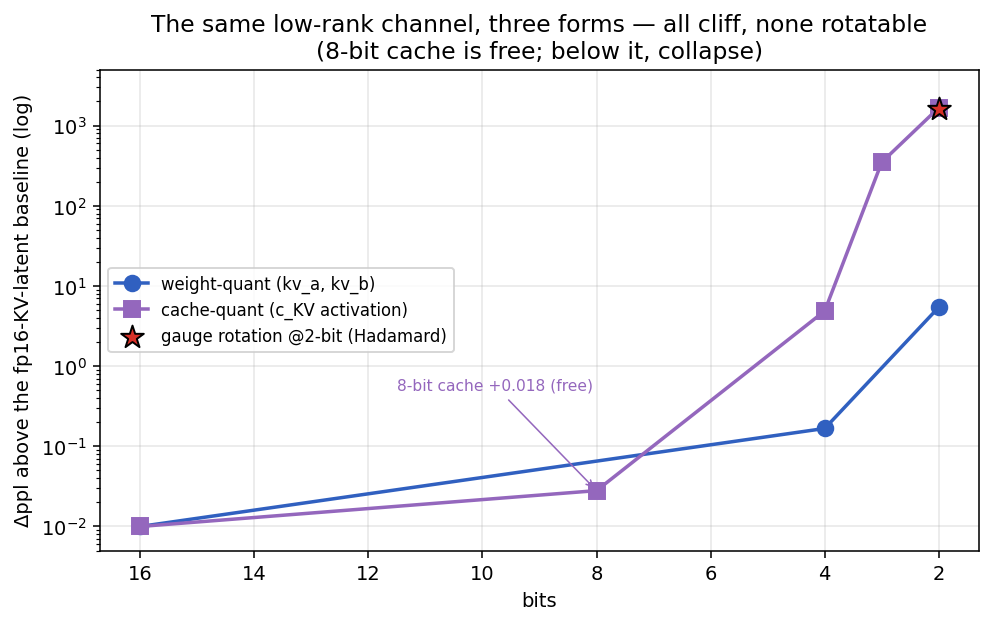
\includegraphics[width=0.72\linewidth]{fig_bottleneck_forms.png}
\caption{The same low-rank channel in three forms (\S\ref{sec:law}): weight-quantization of kv\_a/kv\_b,
quantization of the c\_KV cache activation, and gauge rotation at 2-bit. All cliff and none is rotatable;
the 8-bit cache point is free ($+0.018$), and the cache cliffs at a higher bit-width than the weights.}\label{fig:forms}
\end{figure}

\begin{figure}[t]\centering
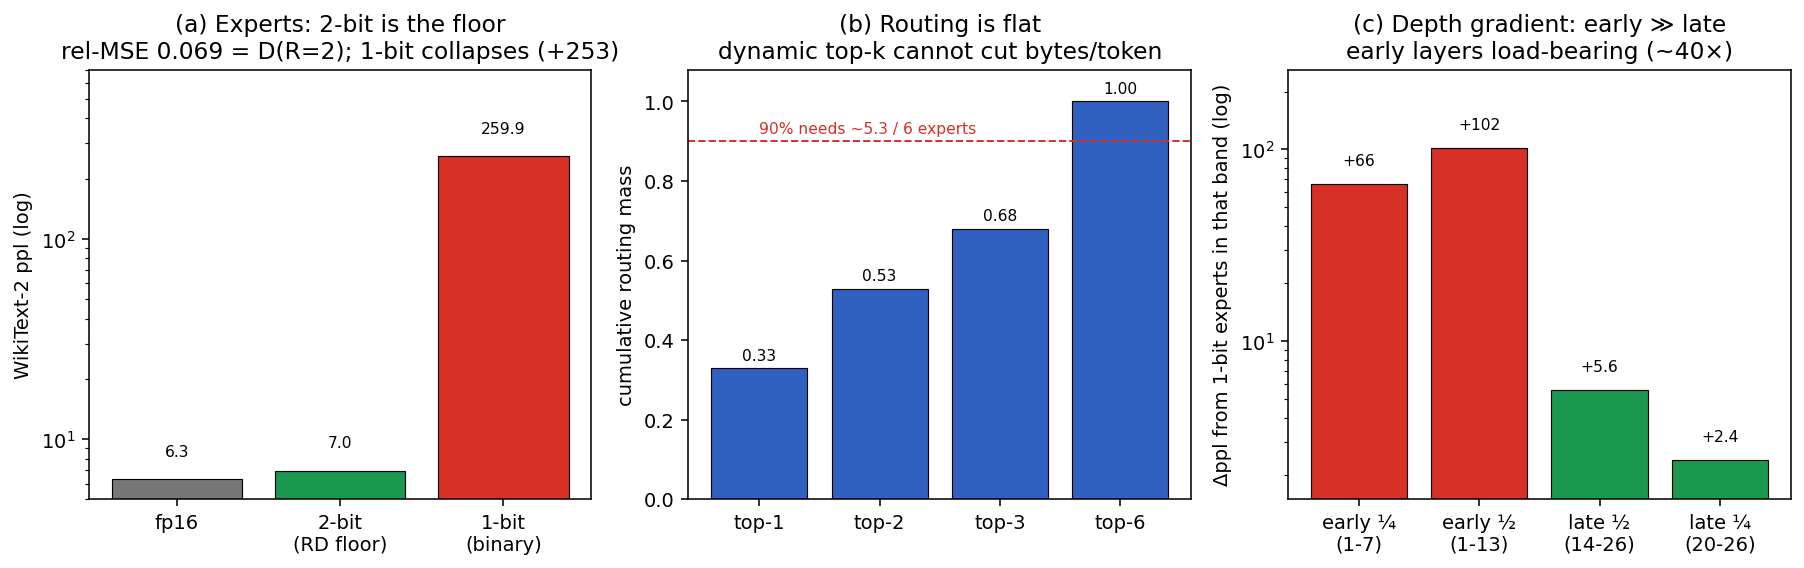
\includegraphics[width=0.97\linewidth]{fig_density.png}
\caption{The density of trained MoEs (\S\ref{sec:density}). \textbf{(a)} Experts: 2-bit is at the Gaussian
RD floor and 1-bit collapses ($+253$). \textbf{(b)} Routing is flat---90\% of the mass needs ${\sim}5.3$ of
6 experts, so dynamic top-k cannot cut bytes/token. \textbf{(c)} Depth gradient: 1-bit experts cost
$+102$ in the early half but $+5.6$ in the late half (${\sim}40\times$).}\label{fig:density}
\end{figure}

% ---------------------------------------------------------------- references
\begin{thebibliography}{99}\small
\bibitem{mxmoe} J.~Chen et al. MxMoE: Mixed-precision Quantization for MoE with Accuracy and Performance
Co-Design. \emph{ICML}, 2025. arXiv:2505.05799.
\bibitem{eaquant} EAQuant: Enhancing Post-Training Quantization for MoE Models via Expert-Aware
Optimization. 2025. arXiv:2506.13329.
\bibitem{mcmoe} W.~Huang et al. MC-MoE: Mixture Compressor for Mixture-of-Experts LLMs Gains More. 2024.
arXiv:2410.06270.
\bibitem{sinq} SINQ: Sinkhorn-Normalized Quantization for Calibration-Free Low-Precision LLM Weights.
2025. arXiv:2509.22944.
\bibitem{qtip} A.~Tseng, Q.~Sun, D.~Hou, C.~De~Sa. QTIP: Quantization with Trellises and Incoherence
Processing. \emph{NeurIPS}, 2024. arXiv:2406.11235.
\bibitem{quip} A.~Tseng, J.~Chee, Q.~Sun, V.~Kuleshov, C.~De~Sa. QuIP\#: Even Better LLM Quantization
with Hadamard Incoherence and Lattice Codebooks. \emph{ICML}, 2024. arXiv:2402.04396.
\bibitem{awq} J.~Lin et al. AWQ: Activation-aware Weight Quantization for LLM Compression and
Acceleration. \emph{MLSys}, 2024. arXiv:2306.00978.
\bibitem{gptq} E.~Frantar, S.~Ashkboos, T.~Hoefler, D.~Alistarh. GPTQ: Accurate Post-Training
Quantization for Generative Pre-trained Transformers. \emph{ICLR}, 2023. arXiv:2210.17323.
\bibitem{hqq} H.~Badri, A.~Shaji. Half-Quadratic Quantization of Large Machine Learning Models. Mobius
Labs technical report, 2023.
\bibitem{deepseekv2} DeepSeek-AI. DeepSeek-V2: A Strong, Economical, and Efficient Mixture-of-Experts
Language Model. 2024. arXiv:2405.04434.
\bibitem{qwenmoe} Qwen Team. Qwen1.5-MoE: Matching 7B Model Performance with 1/3 Activated Parameters.
Technical report, 2024.
\bibitem{llamacpp} G.~Gerganov et al. llama.cpp. \url{https://github.com/ggml-org/llama.cpp}, 2023--.
\end{thebibliography}

\end{document}
